\documentclass[conference]{IEEEtran}
\usepackage{amsmath}
\usepackage{cite}
\usepackage{graphicx}
\usepackage{booktabs}
\usepackage{array}
\usepackage{url}
\usepackage{subcaption}
\usepackage{breakurl}
\usepackage{epstopdf}
\usepackage{tabularx}
\usepackage{placeins}
\usepackage{float}
\usepackage{titlesec}
\usepackage{newtxtext}
\usepackage{newtxmath}

\titlespacing{\section}{0pt}{6pt}{4pt}
\titlespacing{\subsection}{0pt}{5pt}{3pt}
\titlespacing{\subsubsection}{0pt}{4pt}{2pt}

\title{GROUP\_14\_Experiment: 5\\Design of Current Mirror Using BC547B Transistors}

\author{
    \IEEEauthorblockA{Siddhant Shah (B23334) *, Akash Goel(B23032) †, 
                      Om Maheshwari (B23089) ‡, and Somya Bhadada (B23052) §}
* b23334@students.iitmandi.ac.in \\
† b23032@students.iitmandi.ac.in \\
‡ b23089@students.iitmandi.ac.in \\
§ b23052@students.iitmandi.ac.in}
\date{}

\begin{document}

\maketitle

\begin{abstract}
This paper presents the design methodology of a current mirror circuit using a BC547B transistor.
\end{abstract}

\begin{IEEEkeywords}
Current Mirror, BC547B, Bipolar Junction Transistor (BJT), Reference Current, Current Matching
\end{IEEEkeywords}


\section{Apparatus Required}
\begin{itemize}
    \item \textbf{BC547B NPN Transistor:} 
    \begin{itemize}
        \item Description: General-purpose NPN bipolar junction transistor (BJT) in a TO-92 package with 3-pin configuration (Collector, Base, Emitter).
        \item Specifications: See Table~\ref{tab:bc547_specs} for detailed electrical characteristics \cite{BC547_Datasheet}.
        \begin{table}[h]
            \centering
            \begin{tabular}{ll}
                \toprule
                \textbf{Parameter} & \textbf{Value} \\
                \midrule
                Current gain ($\beta$) & 110–800 (typical $\approx$ 100) \\
                Collector current (I$_C$) & 100 mA maximum \\
                Collector-emitter voltage (V$_{CE}$) & 45V maximum \\
                Emitter-base voltage (V$_{EB}$) & 6V maximum \\
                Collector-base voltage (V$_{CB}$) & 50V maximum \\
                Power dissipation & 500 mW maximum \\
                Transition frequency (f$_T$) & 300 MHz \\
                Operating temperature & -65°C to +150°C \\
                Noise figure & Low \\
                Applications & Switching, amplification \\
                \bottomrule
            \end{tabular}
            \caption{BC547B NPN Transistor Specifications.}
            \label{tab:bc547_specs}
        \end{table}
        \begin{figure}[h]
            \centering
            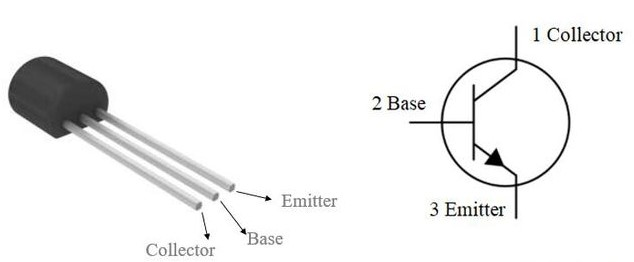
\includegraphics[width=0.3\textwidth]{pinout.jpg} % Replace with actual image file name
            \caption{BC547B NPN Transistor Pinout (TO-92 Package).}
            \label{fig:bc547_pinout}
        \end{figure}
    \end{itemize}

    \item \textbf{Resistors:} 1k$\Omega$.

    \item \textbf{Power Supply:} Keithley 2231A-30-3 (triple output, 30V/3A).

    \item \textbf{Digital Multimeter (DMM):} Agilent 34401A (6$\frac{1}{2}$ digit resolution) for DC measurements.

    \item \textbf{Breadboard and Connectors:} For circuit prototyping.
\end{itemize}



\section{Introduction}
\noindent{The \textbf{Bipolar Junction Transistor (BJT)} is a three-terminal semiconductor device that operates as a current-controlled current source \cite{b1}. It consists of three doped semiconductor regions: the \textbf{Emitter (E)}, \textbf{Base (B)}, and \textbf{Collector (C)}. BJTs are classified into two types: \textbf{NPN} and \textbf{PNP}, depending on the doping arrangement.}

\subsection{Current Mirror}
\noindent{A \textbf{current mirror} is an analog circuit designed to copy (or mirror) a reference current ($I_{REF}$) from one active device (typically a BJT or MOSFET) to another, maintaining a constant output current ($I_{OUT}$) regardless of load variations. It is widely used in analog integrated circuits for biasing and active load purposes \cite{b2}.}

\subsubsection{Basic Principle}
\noindent{The current mirror operates based on the matching characteristics of two transistors. If both BJTs are identical and share the same $V_{BE}$ (base-emitter voltage), then the collector current of the second transistor will mirror that of the first.}

\begin{figure}[htbp]
\centering
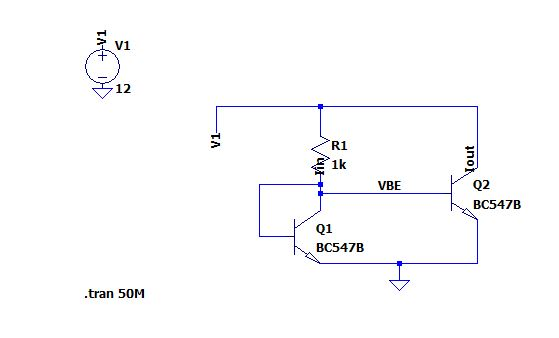
\includegraphics[width=0.4\textwidth]{current_mirror.jpg}
\caption{Basic BJT current mirror circuit using matched NPN transistors \cite{b1}.}
\label{fig:current_mirror}
\end{figure}

\subsubsection{Working}
\begin{itemize}
    \item The reference current $I_{REF}$ flows through transistor $Q_1$ whose collector and base are shorted.
    \item Transistor $Q_2$ shares its base with $Q_1$ and mirrors the same base-emitter voltage ($V_{BE}$).
    \item The reference current $I_{REF}$ is set by the resistor $R$ and is given by:
    \begin{equation}
    I_{REF} = \frac{V_{CC} - V_{BE}}{R}
    \end{equation}
    \item Assuming matched transistors and negligible base current, the output current is:
    \begin{equation}
    I_{OUT} \approx I_{REF} = \frac{V_{CC} - V_{BE}}{R}
    \end{equation}
    \item The accuracy of current mirroring depends on matching of $V_{BE}$, transistor $\beta$, and thermal characteristics.
\end{itemize}

\subsubsection{Small-Signal Behavior}
\noindent{The output impedance of the current mirror is primarily determined by the output resistance of $Q_2$, which increases the mirror's ability to act as a constant current source.}
\begin{equation}
r_o = \frac{V_A}{I_C}
\end{equation}
where $V_A$ is the Early voltage, and $I_C$ is the collector current.

\subsubsection{Applications}
\begin{itemize}
    \item Biasing circuits in analog ICs
    \item Active loads for amplifier stages
    \item Current reference generation
    \item Differential amplifier stages
\end{itemize}

\subsubsection{Advantages}
\begin{itemize}
    \item Provides stable and predictable current source
    \item Simple implementation using BJTs
    \item Reduces the need for large resistors in IC design
\end{itemize}

\subsubsection{Limitations}
\begin{itemize}
    \item Sensitive to transistor mismatches and temperature variations
    \item Limited output compliance range
    \item Finite output impedance affects precision
\end{itemize}

\section{Procedure}
\noindent{The following steps outline the systematic construction, testing, and simulation of the current mirror circuit, using both a physical breadboard setup and LTSpice software. Refer to Figure~\ref{fig:mirror_circuit} for the schematic of the current mirror.}

\begin{enumerate}
    \item \textbf{Component Collection:} Gather the required components: two identical NPN transistors (e.g., BC547B), resistors ($R_{\text{ref}} = 1 \, \text{k}\Omega$, $R_{\text{load}} = 1 \, \text{k}\Omega$), Keithley 2231A-30-3 power supply, Agilent 34401A DMM, breadboard, and connecting wires.

    \item \textbf{Breadboard Assembly:} Construct the current mirror circuit on the breadboard:
    \begin{itemize}
        \item Connect the collector of transistor $Q_1$ to the positive 9 V rail.
        \item Join the base and collector of $Q_1$ together and connect a $1 \, \text{k}\Omega$ resistor ($R_{\text{ref}}$) between this node and ground. This resistor sets the reference current.
        \item Connect the base of $Q_2$ to the base of $Q_1$ (common base node).
        \item Connect the emitter of both transistors to ground.
        \item Attach a $1 \, \text{k}\Omega$ (or even of higher value) load resistor ($R_{\text{load}}$) from the collector of $Q_2$ to the 9 V rail.
    \end{itemize}

    \item \textbf{Power Supply Configuration:} Set the Keithley power supply to provide 12 V DC with a current limit of 50 mA. Connect the positive terminal to the 12 V rail and the negative terminal to the ground rail. Use the Agilent 34401A DMM to verify voltage stability across the rails.

    \item \textbf{Current Verification:} Use the DMM to measure the voltage across $R_{\text{ref}}$ and compute the reference current $I_{\text{ref}} = V_{R_{\text{ref}}} / R_{\text{ref}}$. Similarly, measure the voltage across $R_{\text{load}}$ to compute the output current $I_{\text{out}} = V_{R_{\text{load}}} / R_{\text{load}}$. Verify that $I_{\text{out}} \approx I_{\text{ref}}$, indicating proper mirroring behavior.

    \item \textbf{Performance Under Load:} Vary the value of $R_{\text{load}}$ (e.g., 470 $\Omega$, 2.2 k$\Omega$) and repeat the above measurements to examine the output current regulation. Note that a well-designed current mirror maintains nearly constant $I_{\text{out}}$ despite varying $R_{\text{load}}$.

    \item \textbf{LTSpice Simulation:} Simulate the current mirror using LTSpice:
    \begin{itemize}
        \item Construct the same circuit using BC547B models.
        \item Apply a 12 V DC voltage source.
        \item Use a parameter sweep for $R_{\text{load}}$ and perform a DC operating point analysis.
        \item Observe and plot $I_{\text{ref}}$ and $I_{\text{out}}$ to verify current mirroring and output current constancy.
    \end{itemize}
    \begin{figure}[h]
        \centering
        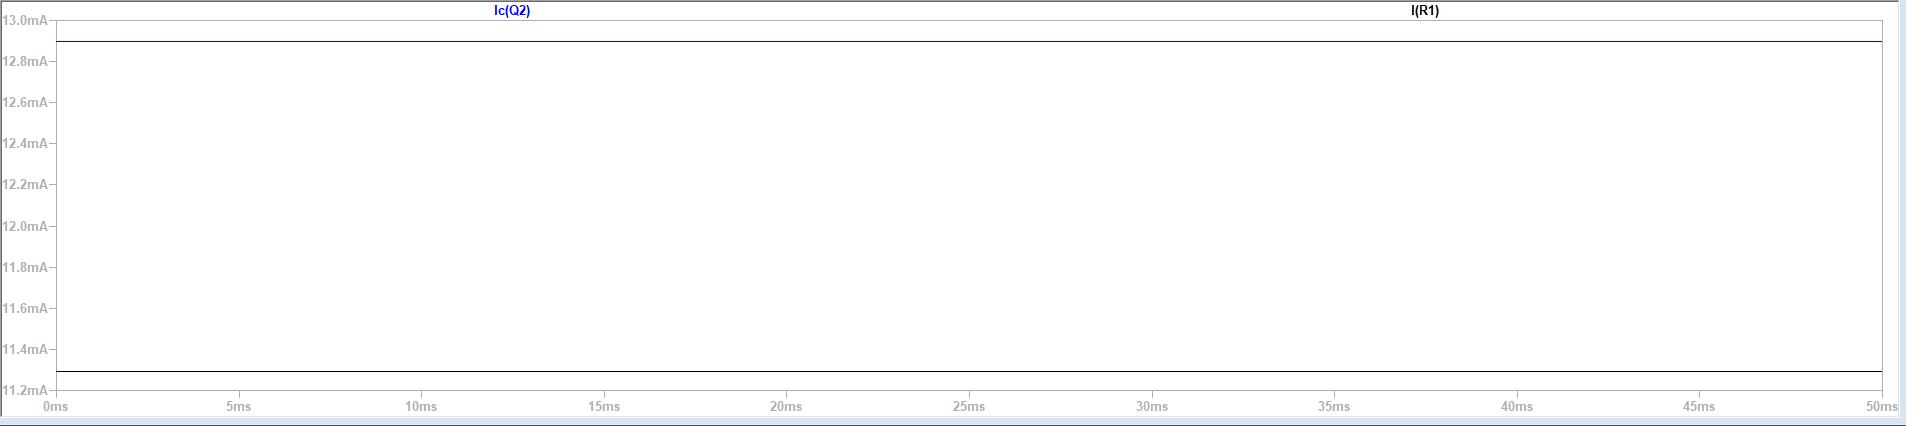
\includegraphics[width=0.5\textwidth]{LTspice_mirror_output.jpg} % Replace with your LTSpice current plot
        \caption{LTSpice output showing current mirroring behavior across $R_{\text{load}}$.}
        \label{fig:mirror_output}
    \end{figure}

    \textbf{NOTE:}  During LTspice simulation we kept the voltage as 12V and we didn't applied a load resistor at $Q_2$ but while performing the experiment you have to take a Load resistor and keep the voltage low not 12V , we kept 9V. The load resistor can be kept high as compared to Reference resistor and it is required at $Q_2$ because we need more voltage drop at $Q_2$ then $Q_1$ then only it will show the output in DMM. Instead of using resistor for voltage drop you can also connect $Q_2$ with different value of voltage source lesser than the voltage source at $Q_1$ in order to get output.

    \item \textbf{Analysis and Validation:} Compare simulated and experimental values of $I_{\text{ref}}$ and $I_{\text{out}}$. Discuss the current matching accuracy and potential sources of mismatch, such as V\textsubscript{BE} differences or Early effect. Validate performance against theoretical expectations.
\end{enumerate}

\section{Results}
\begin{enumerate}
    \item So from the LTspice simulation you can see that when we kept input voltage as 12V we got current on reference resistor to be 11.3mA and current at $Q_2$ 12.8mA. This difference is because we didn't connected the load resistor.
    \item When we performed practically we gave input voltage to $Q_1$ as 9V and $Q_2$ to a lower voltage and compared the result of current at both $Q_1$ and $Q_2$ it wads nearly same. You can see below the images of the circuit and the result in DMM.
    \begin{figure}[h]
        \centering
        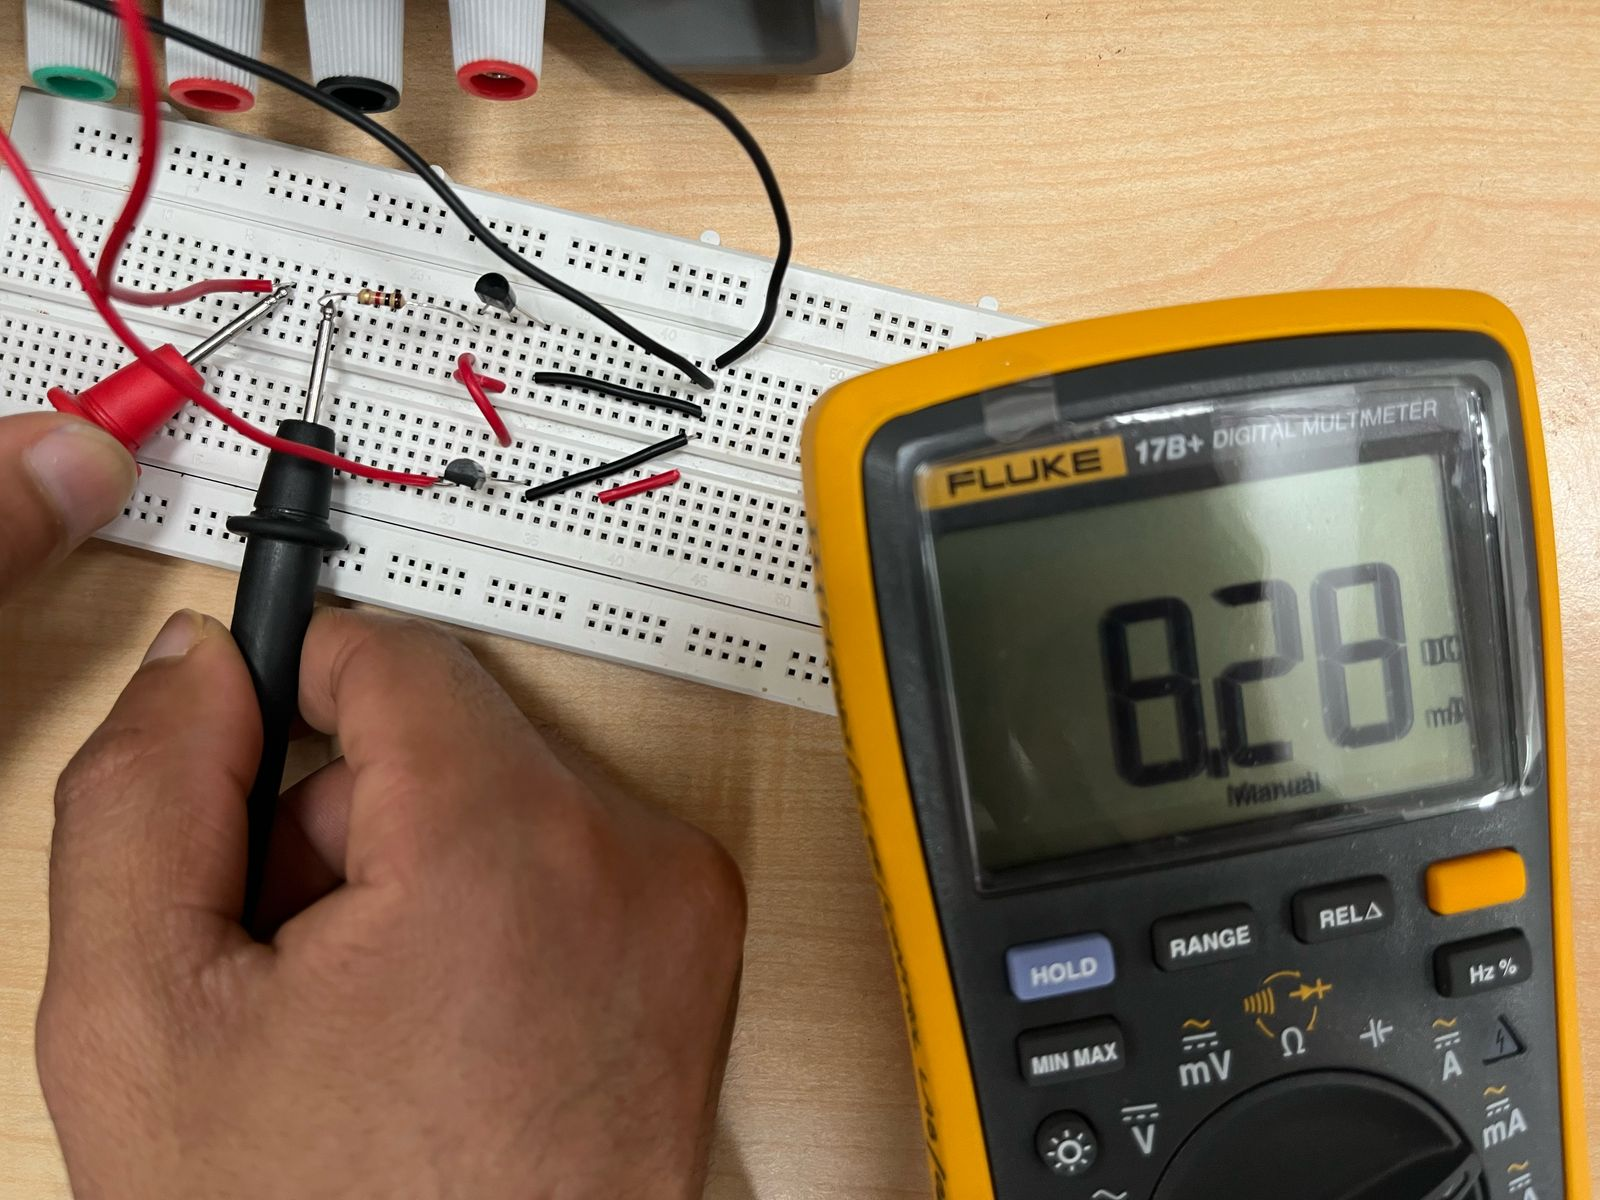
\includegraphics[width=0.5\textwidth]{current_1.jpg} % Replace with your LTSpice current plot
        \caption{Image showing current across $R_{\text{Ref}}$.}
        \label{fig:mirror_output}
    \end{figure}
    \begin{figure}[h]
        \centering
        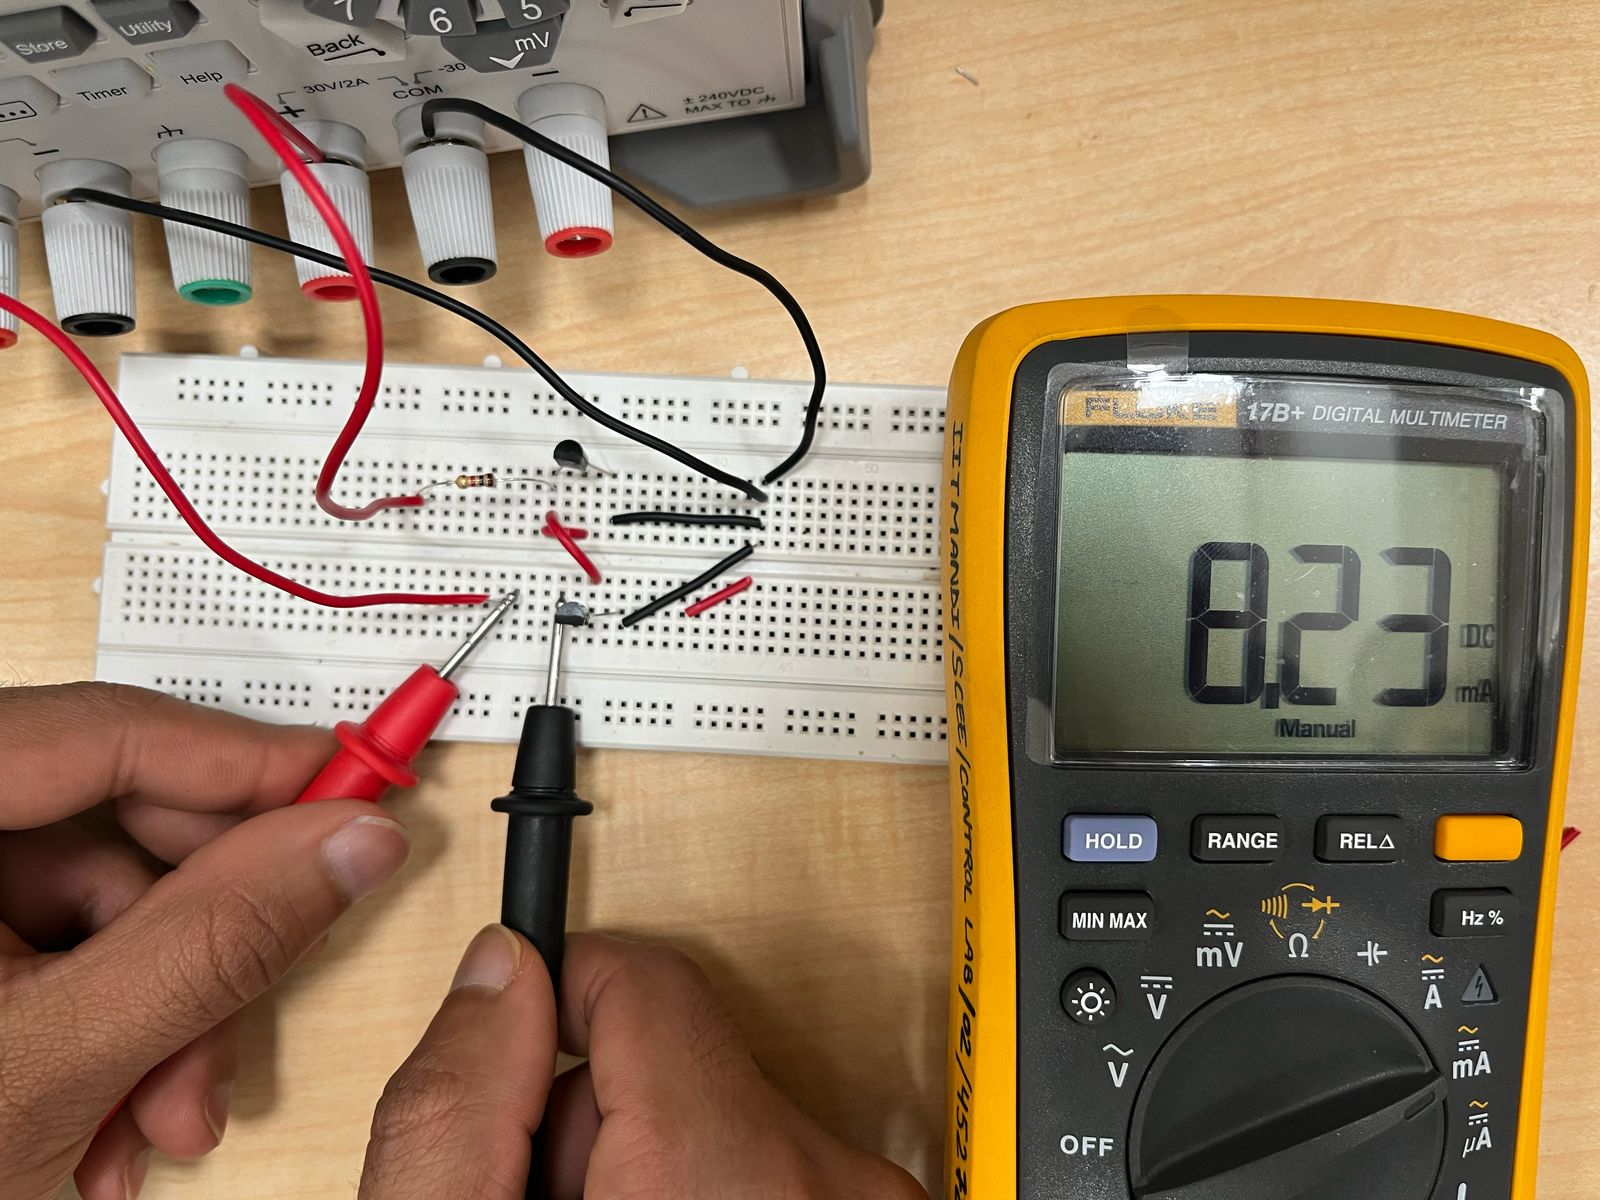
\includegraphics[width=0.5\textwidth]{current_2.jpg} % Replace with your LTSpice current plot
        \caption{Image showing current across $R_{\text{Load}}$.}
        \label{fig:mirror_output}
    \end{figure}
\end{enumerate}

\section{Conclusion}
\noindent{The experiment successfully demonstrated the working principle of a basic current mirror using two matched NPN transistors (BC547B). Both LTSpice simulations and practical breadboard implementations verified that the output current ($I_{\text{out}}$) closely tracks the reference current ($I_{\text{ref}}$), confirming the mirror's ability to replicate current accurately across branches.}\\

\noindent{The circuit maintained a near-constant output current even when different load resistances were used, reflecting the fundamental behavior of current mirrors as active loads or current sources. The results thus validate the theoretical expectations and showcase the reliability of current mirrors in analog circuit applications.}

\section{Discussion}
\noindent{In the LTSpice simulation, the circuit was modeled without a load resistor at the output transistor ($Q_2$), and the supply voltage was set to 12 V. Under these conditions, the output current ($I_{\text{out}}$) slightly exceeded the reference current ($I_{\text{ref}}$). This discrepancy is explained by the Early effect, where differences in the collector-emitter voltage ($V_{\text{CE}}$) influence the output current due to the finite output resistance of the transistor.}\\

\noindent{Practically, the setup used a 9 V supply and included a load resistor at $Q_2$, ensuring a greater voltage drop and bringing $V_{\text{CE}}$ values of both transistors closer. This setup resulted in more accurate current mirroring with $I_{\text{out}} \approx I_{\text{ref}}$. The use of a load resistor also improved visibility of current flow on the DMM, which is critical in practical measurements.}\\

\noindent{Additional observations include:}
\begin{itemize}
    \item \textbf{Transistor Matching:} While identical transistor models were used, manufacturing variations can introduce minor differences in base-emitter voltage ($V_{\text{BE}}$), affecting current accuracy.
    \item \textbf{Compliance Voltage:} The output current remained stable for varying $R_{\text{load}}$, as long as the transistor operated in the active region. However, for very high $R_{\text{load}}$, the output transistor may enter saturation, deviating from ideal behavior.
    \item \textbf{Simulation vs Practical Results:} The practical setup introduced real-world non-idealities such as contact resistance on the breadboard, slight variations in component values, and measurement errors, none of which are accounted for in simulation.
\end{itemize}

\noindent{Overall, this experiment highlights the importance of both simulation and physical implementation when validating analog circuit behavior. It also underscores key design considerations in practical applications of current mirrors, such as matching conditions, supply voltage selection, and output compliance requirements.}

\begin{thebibliography}{9}
\bibitem{b1} A. S. Sedra and K. C. Smith, \textit{Microelectronic Circuits}, 7th ed., Oxford University Press, 2015.
\bibitem{b2} R. Boylestad and L. Nashelsky, \textit{Electronic Devices and Circuit Theory}, 11th ed., Pearson, 2013.

	
    \bibitem{Sedra_Smith}
    A. Sedra, K. Smith, \textit{Microelectronic Circuits}, 7th ed. Oxford University Press, 2014.

    \bibitem{Razavi_Fundamentals}
    B. Razavi, \textit{Fundamentals of Microelectronics}, 2nd ed. Wiley, 2013.

    \bibitem{BC547_Datasheet} 
    ON Semiconductor, "BC547 Datasheet," 2021. [Online]. Available: \url{https://www.onsemi.com/pdf/datasheet/bc547-d.pdf}
    

\end{thebibliography}

\end{document}
